\section{Criterio della massima verosimiglianza - Maximum Likelihood - ML}
Il criterio di stima della massima verosimiglianza \index{Massima Verosimiglianza}\index{Maximum Likelihood} (ML) si basa sulla conoscenza della ddp congiunga $f_X^{(\theta)}(X)$. In letteratura si trova spesso la scrittura $f_X(X|\theta)$ ma è concettualmente errato (al momento) perché si indica una relazione fra $X$ e $\theta$, ma $\theta$ non è una V.C. e la relazione non può quindi sussistere\footnote{una relazione di dipendenza esiste solo fra V.C., mentre $\theta$ è un numero che indica una stima}.\newline
Per un particolare $\bar{\theta}$ e un particolare set di dati $\bar{x}$:

    \[ L(\bar{\theta},\bar{x}):=f_X^{(\bar{\theta})}(\bar{x})=f_X(\bar{x}|\bar{\theta}) \]

La funzione $L$ è detta verosimiglianza di $\bar{\theta}$ sulla base dell'osservazione $\bar{x}$. Per variabili discrete, invece, definiamo la verosimiglianza \index{Verosimiglianza} usando la probabilità congiunta:

    \[ L(\bar{\theta},\bar{x}):=P^{(\bar{\theta})}(X=\bar{x})=P(X=\bar{x}|\theta=\bar{\theta}) \]

\begin{esempio} %###########
Sia data una moneta di cui non conosciamo nulla circa la sua onestà; da alcuni lanci otteniamo $\bar{x}=\{T,T,T,T\}$ e vogliamo ottenere una stima della probabilità che la moneta dia testa $\theta=P(T)$. Calcoliamo ora la verosimiglianza; essendo questo un esperimento discreto scriviamo:

    \[ L(\bar{\theta},\bar{x})=L(\theta,\{T,T,T,T\})=P(\{T,T,T,T\}|\theta)=\theta \cdot \theta \cdot \theta \cdot \theta = \theta^4 \]

Se conoscessimo in anticipo il valore di $\theta=P(T)$, allora potremmo scrivere:

\begin{enumerate}
  \item $\theta=\frac{1}{2}  \Rightarrow L(\theta,x)=\theta^4=\frac{1}{16}$
  \item $\theta=1  \Rightarrow L(\theta,x)=\theta^4=1$
\end{enumerate}

  \begin{figure}[htbp]
      \centering
      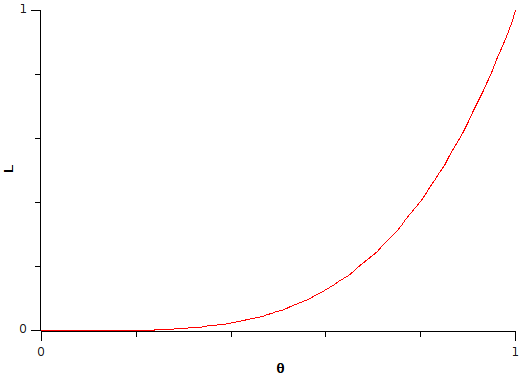
\includegraphics[scale=0.5]{img/verosim.png}
      \caption{Andamento della verosimiglianza\label{fig:verosim1}}
  \end{figure}

La verosimiglianza, come si vede in figura \ref{fig:verosim1}, raggiunge il suo massimo valore nel secondo caso, ovvero per $\theta=1$, il che significa che siamo portati a pensare che la moneta sia truccata e che dia sempre testa.
\end{esempio}

\begin{esempio} %###########
Usiamo ancora la stessa moneta dell'esempio precedente ed otteniamo un differente insieme di dati $\bar{x}=\{T,T,C,C\}$ e quindi la verosimiglianza diventa:

    \[ L(\bar{\theta},\bar{x})=L(\theta,\{T,T,C,C\})=P(\{T,T,C,C\}|\theta)=\theta \cdot \theta \cdot (1-\theta) \cdot (1-\theta) = \theta^2 \cdot (1-\theta)^2 \]

valutiamola quindi per alcuni valori di $\theta$:

\begin{enumerate}
  \item $\theta=1  \Rightarrow L(\theta,x)=\theta^2 \cdot (1-\theta)^2=1 \cdot 0=0$
  \item $\theta=\frac{1}{2}  \Rightarrow L(\theta,x)=\theta^2 \cdot (1-\theta)^2=0.25 \cdot 0.25=0.0625$
  \item $\theta=\frac{1}{10}  \Rightarrow L(\theta,x)=\theta^2 \cdot (1-\theta)^2=0.01 \cdot 0.081=0.0081$
\end{enumerate}

  \begin{figure}[htbp]
    \centering
    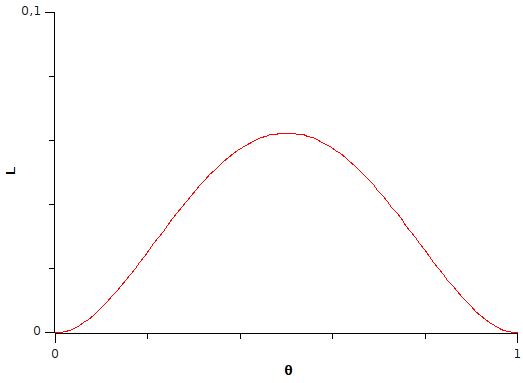
\includegraphics[scale=0.5]{img/verosim2.png} 
    \caption{verosimiglianza\label{fig:verosim2}}
  \end{figure}
La massima verosimiglianza, come si vede in figura \ref{fig:verosim2}, è raggiunta nel secondo caso, per $\theta=\frac{1}{2}$, il che significa che siamo portati a pensare che la moneta sia onesta e che mediamente esca testa la metà delle volte.
\end{esempio}

Dagli esempi si evince che il parametro $\theta$ di cui vogliamo una stima con il criterio della massima verosimiglianza, è dato dal valore che massimizza la funziona di verosimiglianza, quindi:

    \[ \theta^{ML}(X)=\arg \max_{\theta \in D_\theta} L(\theta,X) \]

Da notare che la funzione di verosimiglianza $L$ non è una ddp, ciò che varia è $\theta$ e non $X$, infatti $\theta$ non è nemmeno una V.C. ma un risultato puntuale di una funzione, inoltre, non essendo una V.C:

  \[ \int_{D_\theta}^{}L(\theta,X) d\theta\ne 1 \]
  
Molto spesso massimizzare la verosimiglianza può essere computazionalmente complesso e quindi può essere utile risolvere il problema di massimizzazione del supporto della verosimiglianza\index{Supporto della verosimiglianza}\index{Log likelihood}; ai fini della stima del parametro $\theta$ i metodi sono equivalenti. Definiamo allora il supporto della verosimiglianza (Log likelihood):

  \[ S(\theta,X):= \ln L(\theta,X)  \]
  
e quindi la stima ML diventa:

  \[ \theta^{ML}(X)=\arg \max_{\theta \in D_\theta} S(\theta,X)  \]
  
Un esempio piuttosto comune che rende preferibile la massimizzazione del supporto è dato dall'uso di V.C. iid. Il motivo è che la ddp congiunta di V.C. iid è la produttoria di tutte le ddp, quindi in fase di massimizzazione il calcolo della derivata diventa complesso:

  \[ L(\theta,X)=f_X^{(\theta)}(x)=\prod_{i=1}^{N}  f_{X_i}^{(\theta)}(x)  \]
  
con l'uso del supporto la massimizzazione diventa molto più semplice, infatti:

  \[ S(\theta,X)= \ln L(\theta,X )= \ln \prod_{i=1}^{N}  f_{X_i}^{(\theta)}  =  \sum_{i=1}^{N}   f_{X_i}^{(\theta)} \]
  
Concludiamo con alcune proprietà di cui gode lo stimatore ML. Sotto ipotesi di regolarità, lo stimatore ML, per campioni indipendenti, è uno stimatore asintoticamente: consistente, gaussiano e non polarizzato, inoltre, sempre asintoticamente, raggiunge il limite CR. Ovviamente queste proprità non valgono per piccole quantità di dati.
Sempre sotto ipotesi di regolarità vale:

  \[ \eta = h(\theta^{ML}) \]

\begin{esempio}  
Supponiamo di voler stimare una valore $x^3$, allora:

  \[ h(x)=x^3 \]
  
e quindi possiamo stimare $\theta^{ML} = x$ e poi calcolare:

  \[ \eta^{ML} = h(\theta^{ML})={\theta^{ML}}^3 \]
\end{esempio}

In conclusione, possiamo affermare che la stima ML ha il grande pregio di essere una tecnica molto generale, ma ha un difetto altrettanto grande che dipende dalla conoscenza della ddp congiunta dell'esperimento, il che è difficilmente noto a priori.
